% Options for packages loaded elsewhere
\PassOptionsToPackage{unicode}{hyperref}
\PassOptionsToPackage{hyphens}{url}
%
\documentclass[
]{book}
\usepackage{amsmath,amssymb}
\usepackage{lmodern}
\usepackage{iftex}
\ifPDFTeX
  \usepackage[T1]{fontenc}
  \usepackage[utf8]{inputenc}
  \usepackage{textcomp} % provide euro and other symbols
\else % if luatex or xetex
  \usepackage{unicode-math}
  \defaultfontfeatures{Scale=MatchLowercase}
  \defaultfontfeatures[\rmfamily]{Ligatures=TeX,Scale=1}
\fi
% Use upquote if available, for straight quotes in verbatim environments
\IfFileExists{upquote.sty}{\usepackage{upquote}}{}
\IfFileExists{microtype.sty}{% use microtype if available
  \usepackage[]{microtype}
  \UseMicrotypeSet[protrusion]{basicmath} % disable protrusion for tt fonts
}{}
\makeatletter
\@ifundefined{KOMAClassName}{% if non-KOMA class
  \IfFileExists{parskip.sty}{%
    \usepackage{parskip}
  }{% else
    \setlength{\parindent}{0pt}
    \setlength{\parskip}{6pt plus 2pt minus 1pt}}
}{% if KOMA class
  \KOMAoptions{parskip=half}}
\makeatother
\usepackage{xcolor}
\usepackage{longtable,booktabs,array}
\usepackage{calc} % for calculating minipage widths
% Correct order of tables after \paragraph or \subparagraph
\usepackage{etoolbox}
\makeatletter
\patchcmd\longtable{\par}{\if@noskipsec\mbox{}\fi\par}{}{}
\makeatother
% Allow footnotes in longtable head/foot
\IfFileExists{footnotehyper.sty}{\usepackage{footnotehyper}}{\usepackage{footnote}}
\makesavenoteenv{longtable}
\usepackage{graphicx}
\makeatletter
\def\maxwidth{\ifdim\Gin@nat@width>\linewidth\linewidth\else\Gin@nat@width\fi}
\def\maxheight{\ifdim\Gin@nat@height>\textheight\textheight\else\Gin@nat@height\fi}
\makeatother
% Scale images if necessary, so that they will not overflow the page
% margins by default, and it is still possible to overwrite the defaults
% using explicit options in \includegraphics[width, height, ...]{}
\setkeys{Gin}{width=\maxwidth,height=\maxheight,keepaspectratio}
% Set default figure placement to htbp
\makeatletter
\def\fps@figure{htbp}
\makeatother
\setlength{\emergencystretch}{3em} % prevent overfull lines
\providecommand{\tightlist}{%
  \setlength{\itemsep}{0pt}\setlength{\parskip}{0pt}}
\setcounter{secnumdepth}{5}
\usepackage{booktabs}
\usepackage{amsthm}
\makeatletter
\def\thm@space@setup{%
  \thm@preskip=8pt plus 2pt minus 4pt
  \thm@postskip=\thm@preskip
}
\makeatother
\usepackage{booktabs}
\usepackage{longtable}
\usepackage{array}
\usepackage{multirow}
\usepackage{wrapfig}
\usepackage{float}
\usepackage{colortbl}
\usepackage{pdflscape}
\usepackage{tabu}
\usepackage{threeparttable}
\usepackage{threeparttablex}
\usepackage[normalem]{ulem}
\usepackage{makecell}
\usepackage{xcolor}
\ifLuaTeX
  \usepackage{selnolig}  % disable illegal ligatures
\fi
\usepackage[]{natbib}
\bibliographystyle{apalike}
\IfFileExists{bookmark.sty}{\usepackage{bookmark}}{\usepackage{hyperref}}
\IfFileExists{xurl.sty}{\usepackage{xurl}}{} % add URL line breaks if available
\urlstyle{same} % disable monospaced font for URLs
\hypersetup{
  pdftitle={Non-stationary spatial distribution models, and its application in marine megafauna.},
  pdfauthor={Martina Le-Bert Heyl},
  hidelinks,
  pdfcreator={LaTeX via pandoc}}

\title{Non-stationary spatial distribution models, and its application in marine megafauna.}
\author{Martina Le-Bert Heyl}
\date{2024-01-28}

\begin{document}
\maketitle

{
\setcounter{tocdepth}{1}
\tableofcontents
}
\hypertarget{introduction}{%
\chapter*{Introduction}\label{introduction}}
\addcontentsline{toc}{chapter}{Introduction}

The availability of spatial methods in statistics has increased substantially in the past decades due to advances in sampling tools as-well-as computational efforts to analyze it. Some examples include data collected from drones, and satellite images \citep{perry_illustrations_2002, pettorelli_satellite_2014}, and software development like arcgis \citep{scott_spatial_2010} or specialized R packages \citep{r-core_comprehensive_2000}. Spatial analysis has become essential for many intriguing questions in fields ranging from epidemiology to ecology \citep{fortin_spatial_2006, fotheringham_local_1999, moraga_spatial_2023}. However, non of it comes without its challenges, learning from the data requires statistical models that can resemble reality. This is of particular importance when studying phenomena or patterns at a local scale.

Models used then should allow researchers to take into account all available information including spatial correlation. Many ecological datasets exhibit spatial correlation in the observed variables due to biotic or abiotic processes, such as dispersal limitation, social aggregation, and spatial structure in unobserved explanatory variables. Whether the observations are points in space (e.g., the location of an endangered species), counts (e.g., the number of individuals of the endangered species in the sample space), or values of some continuous variable (e.g., water nutrient levels at sampled points), spatial correlation means that each observation depends on any other observation within some unknown range of correlation. Unlike models assuming independence between observations, Bayesian inference models allow us to consider spatial correlation.

For this reason, the implementation of spatially explicit Bayesian models has received increasing attention. In other words, it is becoming more and more necessary for researchers to use Bayesian inference as a tool to deal with georeferenced data.

In this introductory section a brief review on the following is given, i) Bayesian theory and computation; ii) Integrated Nested Laplace Approximation (INLA); iii) Stochastic Partial Differential Equations (SPDE), and iv) point processes. Although the entirety of the project doesn't intend to profoundly do research on these topics a preliminary discussion on it is necessary to understand the proposed model and applications later on.

\hypertarget{bayesian-theory-and-computation}{%
\section*{Bayesian Theory and computation}\label{bayesian-theory-and-computation}}
\addcontentsline{toc}{section}{Bayesian Theory and computation}

A starting point in Bayesian analysis is the consideration of parameters \(\theta\) as random variables in contrast to the frequentist perspective, which treats parameters as fixed but unknown values. Then, knowledge about \(\theta\) comes from the distribution of \(\theta\) given the data \(y\). Getting this distribution is done using Bayes theorem.

\[\pi(\theta|y)=\frac{\pi(y|\theta)\pi(\theta)}{\pi(y)}\]

In the equation, \(\pi(\theta|y)\) is the \emph{posterior} distribution of \(\theta\) given the data \(y\); \(\pi(y|\theta)\) is the likelihood of the data \(y\) given \(\theta\); \(\pi(\theta)\) is \emph{prior} density function for \(\theta\); and \(\pi(y)\) is the marginal likelihood of \(y\) that acts as a normalizing constant. The latter is often hard to obtain so Bayes theorem is simplified to,

\[\pi(\theta|y)\propto\pi(y|\theta)\pi(\theta)\]
In the previous equations \(\pi(\theta|y)\) is actually the \emph{joint posterior} distribution. To obtain individual an parameter the \emph{marginal posterior} for that parameter has to be calculated. This is done by integrating \(\theta_{-i}\) parameters out, \(\theta_{i}\) being the parameter of interest.

\[\pi(\theta_{i}|y)=\int\pi(\theta|y)d\theta_{-i}\]
with, \(i=1,...,dim(\theta)\).

Bayesian theory is clear, but the calculation of posterior densities can be computationally intensive. The following describes random sampling and approximation methods for computation in Bayesian statistics.

\textbf{Sampling:} The goal of methods based on random sampling is to generate and sample posterior distributions arbitrarily. The main sampling methods are based on generating a Markov chain whose stationary distribution is the posterior distribution. Collectively, these methods are known as Markov Chain Monte Carlo (MCMC) \citep{gelfand_sampling-based_1990, hastings_monte_1970}. Considering the differences among algorithms implementing the MCMC method, including the Metropolis-Hastings, Gibbs, and Hamiltonian Monte Carlo algorithms \citep{hastings_monte_1970, neal_how_2012, smith_bayesian_1993}, in general:

\begin{enumerate}
\def\labelenumi{\arabic{enumi}.}
\tightlist
\item
  Specify the model and chosen prior distribution.
\item
  Specify the initial values of the chain.
\item
  Let the chain run until it reaches a stationary state. All observations before this point are discarded as warm-up values.
\item
  Obtain the posterior distribution from the sampling.
\end{enumerate}

For each step, there are certain constraints that can make this analysis quite complex and extensive. For example, observations from the chain are positively correlated, so the sampling from the posterior distribution generated by the chain must be large enough to discard dependence. The fact that the posterior distribution comes from sampling means that a sufficient number of samples must be generated for the estimation to be accurate, which can be time-consuming.

\textbf{Approximation:} These methods originated with the article by Tierney and Kadane \citep{tierney_accurate_1986}. Among them, but more recent, is the method of Integrated Nested Laplace Approximation (INLA) \citep{rue_approximate_2009}. The main idea in this case is to obtain the marginal posterior of the parameters \(\pi(\theta_i|y)\) instead the joint posterior.

\hypertarget{inla}{%
\section*{INLA}\label{inla}}
\addcontentsline{toc}{section}{INLA}

Three key components are required by INLA: the latent Gaussian models (LGM) framework, a Gaussian Markov random field (GMRF) \citep{rue_gaussian_2005}, and the Laplace approximation. A brief explanation of these followed by the INLA-SPDE method is given here \citep{krainski_advanced_2018, lindgren_explicit_2011}.

\hypertarget{lgm}{%
\subsection*{LGM}\label{lgm}}
\addcontentsline{toc}{subsection}{LGM}

A three-stage hierarchical model formulation is obtained as follows:

\[\mathrm{y} \mid \mathrm{x}, \theta_1 \sim \prod_{i \in \mathcal{I}} \pi\left(y_i \mid x_i, \theta_1\right)\]
In this first equation \(\mathrm{x}\) is a Gaussian random field, \(\theta_1\) hyperparameters, and \(\mathrm{y}\) independent of observations given \(\mathrm{x}\), and \(\theta_1\).

\[\mathrm{x} \mid \theta_2 \sim \mathcal{N}\left(\mu\left(\theta_2\right), \mathrm{Q}^{-1}\left(\theta_2\right)\right)\]
In the second equation \(\theta_2\) are hyperparameters for the latent GMRF structure of the model,

\[\pi(\mathrm{x}, \theta \mid \mathrm{y}) \propto \pi(\theta) \pi(\mathrm{x} \mid \theta) \prod_{i \in \mathcal{I}} \pi\left(y_i \mid x_i, \theta\right)\]

Finally, in the third equation \(\theta=(\theta_1, \theta_2)\). This equation comes from \(\pi(\mathbf{x}, \theta \mid \mathbf{y}) \propto \pi(\mathbf{x},\theta) \pi(\mathbf{y} \mid \mathbf{x}, \theta)\), where the joint distribution \(\pi(\mathbf{x}, \theta)\) is rearrange as \(\pi(\theta) \pi(\mathrm{x} \mid \theta)\), and \(\pi(\mathbf{y}|\mathbf{x},\theta)\) as \(= \prod_{i \in \mathcal{I}} \pi\left(y_i \mid x_i, \theta\right)\).

There is a few assumptions needed to be considered for the vector of hyperparameters \(\mathbf{\theta}\). 1) the number of hyperparameters is small; 2) as mentioned, the distribution of the latent field \(\mathbf{x}|\mathbf{\theta}\) is a GMRF; 3) the observations \(\mathbf{y}\) are mutually conditional independent of \(\mathbf{x}\) and \(\mathbf{\theta}\). These are assumptions for LGMs also hold for the generalized linear models setup described next.

LGMs can be placed in a generalized linear models setup. The likelihood \(\pi\left(y_i \mid x_i, \theta\right)\) is interpreted so that \(y_i\) only depends on its linear predictor \(x_i\), then \(\left\{x_i, i \in \mathcal{I}\right\}\) is interpreted as the linear predictor \(\eta_i\),

\[\eta_i=\mu+\sum_j \beta_j z_{i j}+\sum_k f_{k, j_k(i)}\]
where \(\mu\) is the overall intercept, \(\mathbf{z}\) fixed covariates with linear effects \({\beta_j}\), and \(f_{k}\) model components in which \(j\) contributes to the \(i\)th linear predictor. \emph{()} give examples of model components \(f_{k}\) and its assumptions.

When Gaussian priors for the intercept and the parameters of the fixed effects are assumed, the joint distribution of \(\mathrm{x}\) is Gaussian,

\[\mathrm{x}=\left(\eta, \mu, \beta, \mathrm{f}_1, \mathrm{f}_2, \ldots\right)\]
\(\mathrm{x}\) is the latent field in the LGM formulation meaning it has a GMRF structure, and observations are considered independent under \(\mathbf{x}\). In this setup the vector of hyperparameters \(\mathbf{\theta}\) contains the parameters from the likelihood and model components.

\hypertarget{gmrf}{%
\subsection*{GMRF}\label{gmrf}}
\addcontentsline{toc}{subsection}{GMRF}

A GMRF is a multivariate Gaussian random variable with additional properties of conditional independence (also called the ``Markov property''): \(x_i\) and \(x_j\) are conditionally independent given the remaining elements if and only if the entry \((i,j)\) of the precision matrix is 0. The sparsity of the precision matrix is a key property for computational efficiency so the latent field should not only be Gaussian but also a GMRF for the INLA method to be efficient.

As LGMs, GMRF can also be constructed additively. As mentioned before \(\mathbf{x}\) is GMRF with precision matrix as result of the sum of the precision matrices of the fixed effects and model components.

Besides counting with sparse matrices, treating \(\mathbf{x}\) as a GMRF has also advantages in the approximation of this joint posterior distribution.

\hypertarget{laplace-approximation}{%
\subsection*{Laplace Approximation}\label{laplace-approximation}}
\addcontentsline{toc}{subsection}{Laplace Approximation}

The Laplace approximation is used to approximate the integral \(I_n=\int_x \exp (n f(x)) d x\) as \(n{\rightarrow}\infty\) by doing a Taylor expansion on \(f(x)\) at its mode \(x_0\).

\[\begin{aligned}
I_n & \approx \int_x \exp \left(n\left(f\left(x_0\right)+\left(x-x_0\right) f^{\prime}\left(x_0\right)+\frac{1}{2}\left(x-x_0\right)^2 f^{\prime \prime}\left(x_0\right)\right)\right) d x \\
& =\exp \left(n f\left(x_0\right)\right) \int \exp \left(\frac{n}{2}\left(x-x_0\right)^2 f^{\prime \prime}\left(x_0\right)\right) d x \\
& =\exp \left(n f\left(x_0\right)\right) \sqrt{\frac{2 \pi}{-n f^{\prime \prime}\left(x_0\right)}}=I_n
\end{aligned}\]

with \(f^{\prime}(x_0)\) and \(f^{\prime\prime}(x_0)\) the first and second order derivatives at \(x_0\). Then, \(I_n\) is the Gaussian integral and \(f^{\prime}(x_0) = 0\). If \(nf(x)\) is taken to be the sum of log-likelihoods, \(x\) the unknown parameter, and the central limit theorem holds, the approximation will be exact as \(n{\rightarrow}\infty\).

In INLA this approximation is used to some of the posterior distributions, for example joint posterior distribution of the hyperparameters \(\pi\left(\theta\mid \mathbf{y}\right)\).

\hypertarget{spde}{%
\section*{SPDE}\label{spde}}
\addcontentsline{toc}{section}{SPDE}

Gaussian random fields (GRFs) are a widely used tool for capturing dependency in spatial modeling. GRFs have the advantage of being fully characterized by its mean and covariance, the latter has a parametrized structure often from the Matérn covariance family, with the parameters termed hyperparameters. However, some computational challenges have to be overcome to estimate the covariance matrix \(\mathbf{\Sigma}\). With INLA, computational speed and accuracy comes from the sparse precision matrix representation \(\mathbf{Q}\). As mentioned before the precision matrix is the inverse of the covariance matrix, then \(\mathbf{Q} = \mathbf{\Sigma}^{-1}\). In the spatial statistics context sparsity is attained using the SPDE approach.

The SPDE approach constructs a continuously indexed approximation of the GRF by using an SPDE model instead of a discrete model on a set on a grid. The following is a brief summary on the intuition behind the SPDE approach.

\hypertarget{matuxe9rn-covariance-function-and-spde}{%
\subsection*{Matérn covariance function and SPDE}\label{matuxe9rn-covariance-function-and-spde}}
\addcontentsline{toc}{subsection}{Matérn covariance function and SPDE}

The use of a Matérn covariance function is convenient as its parameters have a clear physical interpretation. However, covariance matrices calculations are not computationally efficient. The Matérn covariance function is given by,

\[Cov\left(x(s_i), x(s_j)\right)=\sigma^2 \frac{2^{1-\nu}}{\Gamma(\nu)}\left(\sqrt{8 \nu}\left\|s_i-s_j\right\| / \rho\right) K_\nu\left(\sqrt{8 \nu}\left\|s_i-s_j\right\| / \rho\right)\]

where \(||s_i-s_j||\) is the Euclidean distance between points \(s_i\) and \(s_j\), \(\sigma^2\) is the marginal standard deviation, \(\nu\) is the smoothness parameter, \(K_{\nu}\) is the modified Bessel function of the second kind and order \(\nu>0\), and \(\rho\) is the spatial distance at which correlation is approximately 0.1.

In parallel, results from Whittle \citep{whittle_stationary_1954} show that the stationary solution of an SPDE of the following form

\[\left(\kappa^2-\Delta\right)^{\alpha / 2}(\tau x(s))=\mathcal{W}(s), \quad s \in \mathbb{R}^d\]

has a Matérn covariance function representation. In the equation, \(x(s)\) is a GRF, \(\Delta=\sum_i \partial^2 / \partial s_i^2\) is the Laplacian operator and \(\mathcal{W}\) is some Gaussian white noise. Parameters \(\kappa>0\), and \(\boldsymbol{a}>d / 2\) are scale, and smoothness parameters, and \(\boldsymbol{\tau}>0\) controls the variance.

Parameters used in the two previous equations are not the same, however there is a one-to-one correspondence between them. In other words, provided some restrictions on the SPDE, there is an approximation to the solution that is continuously indexed and has the Matérn covariance structure approximately.

\hypertarget{fem}{%
\subsection*{FEM}\label{fem}}
\addcontentsline{toc}{subsection}{FEM}

Without getting into too much detail the Finite Element Method (FEM) is employed to solve the Stochastic Partial Differential Equation (SPDE), which allows solutions to be approximated in an irregular grid. In this case the spatial domain is divided into a set of non-intersecting triangles creating a triangulated mesh with \(n\) nodes or triangle vertices. For each mesh node there is a basis function \(\Psi_k\) which is in turn a piece wise linear function. The approximation is as follows,

\[x(\mathbf{s})=\sum_{k=1}^n \psi_k(\mathbf{s}) w_k\]
Here, the continuously indexed GRF \(x(s)\) is represented as a (discretely indexed) GMRF by a sum of \(\psi_k\) basis functions and \(w_k\) Gaussian distributed weights, with \(k=1,...,n\). The solution preserves the sparsity of the precision matrix for the random field at mesh nodes by carefully choosing the basis functions.

\hypertarget{projection-matrix}{%
\subsection*{Projection matrix}\label{projection-matrix}}
\addcontentsline{toc}{subsection}{Projection matrix}

Now, from the implementation point of view a projection matrix \(\mathbf{A}\) is used in INLA to project observations to the triangles nodes in the mesh. Each row in \(\mathbf{A}\) corresponds to an observation \(i\) at location \(s_i\), and each column to a mesh node. Values in \(\mathbf{A}\) are given by the location \(s_i\) of the observation in the mesh. If the location \(s_i\) lies inside a triangle the \(i\)th row of \(\mathbf{A}\) will have three non-zero entries in the columns of \(\mathbf{A}\) corresponding to the three nodes that construct the triangle where \(s_i\) lies in. If \(s_i\) lies along the edge of a triangle there will be two non-zero entries in the \(i\)th row of \(\mathbf{A}\); and if \(s_i\) is on top of a triangle node there will be just one non-zero entry. Finally each row in \(\mathbf{A}\) sums up to 1.

Finally, since \(x(s)\) is a GRF, a vector of any set of locations will be a multivariate Gaussian vector. The vector's covariance matrix according to the SPDE approximation is,

\[\mathbf{\Sigma}=\mathbf{AQ^{-1}A^{T}}\]

As mentioned in the beginning, this section only intends to give some broad intuition behind Bayesian computation and INLA methods. A detailed explanation can be found in \citet{bakka_non-stationary_2019}; \citet{krainski_advanced_2018}; \citet{lindgren_explicit_2011}; \citet{rue_approximate_2009}; \citet{rue_gaussian_2005}; \citet{simpson_going_2016}.

\hypertarget{point-processes}{%
\section*{Point processes}\label{point-processes}}
\addcontentsline{toc}{section}{Point processes}

A point pattern refers to the arrangement or distribution of individual points or locations within a study area. These points represent the sampled elements or observations in the context of spatial data. Point patterns are commonly encountered in various fields, such as ecology, epidemiology, forestry, and geography, where the goal is to understand the spatial distribution of events or phenomena.

In point processes modelling it is assumed the occurrence of observed events is influenced by an inherent spatial process. The underlying process is modeled using an intensity function \(\lambda(s)\), which it is taken to be the intensity of a Poisson process.

Particularly, a Log-Gaussian Cox Process (LGCP) is a statistical model used for analyzing the distribution of events or occurrences in continuous space.

More in detail, the Cox process is a type of point process that describes the occurrence of events over a continuous spatial domain. It is characterized by an intensity function, which represents the expected number of events per unit area.

The following equation illustrates the number of events in a region \(A\) follow a Poisson process with intensity \(\lambda_A\).

\[\lambda_A=\int_A\lambda(s)ds\]

In the LGCP, the intensity function of the Cox process is log-transformed. Conditional on a set of hyper-parameters, the logarithm of the intensity function is then assumed to follow a Gaussian distribution.

The Gaussian process is used to model the spatial variation in the log-intensity function. It is a stochastic process where the values at any finite set of locations are jointly Gaussian distributed. Then, \(log\lambda(s) = Z(s)\), and \(Z(s)\) a Gaussian process. Moreover, an LGCP is an inhomogeneous Poisson process, conditional on a realization of \(Z(s)\)

Additionally, \citet{simpson_going_2016} developed a method for fitting LGCP models considering an SPDE approach. Because of it it is possible to fit an LGCP model over a mesh instead of a regular grid.

\hypertarget{transparent-barrier-model}{%
\chapter{Transparent Barrier model}\label{transparent-barrier-model}}

\hypertarget{motivation}{%
\section{Motivation}\label{motivation}}

Traditional spatial statistics rely on stationary models like the Matérn field, but they can smooth over features such as boundaries, holes, or physical barriers. For such cases \citet{bakka_non-stationary_2019} proposed the Barrier model as a solution which differs from established methods in the sense that it doesn't rely on the shortest distance between two points for the construction of the covariance matrix function. The Barrier model is based on interpreting the Matérn correlation as a collection of paths through a Simultaneous Autoregressive (SAR) model, manipulating local dependencies to cut off paths crossing physical barriers and formulated as a stochastic partial differential equation (SPDE) for well-behaved discretization.

Until now only \emph{permanent physically impermeable} barriers have been considered in the model. However this turns out to be quite restrictive since some barriers tend to have some degree of \emph{transparency} instead of being permanently impermeable. So a Transparent Barrier model is proposed when barriers with different transparency levels need to be included in the same model. To illustrate this, one can think of some fish that leaves in shallow sea waters. An impermeable barrier would be a set of islands where there is no scenario in which fishes go over it \emph{- we will refer to this as 0 transparency later on -}. However, there might be sand patches with varying water coverage depending on the tide. These sand patches cannot be considered \emph{permanently impermeable} barriers as fishes will be present, but will do so less often than in the \emph{normal} non barrier area. Then, there is the need of counting with a model that can include both barriers and their specific transparency level as some parameter in the model. Moreover, the Barrier model is the case where all the barrier areas have the same transparency level equal to \(0\) in the Transparent Barrier model framework.

The main advantage of the Transparent Barrier model is it can handle spatial structures with complex barriers of different nature while keeping the computational efficiency of the stationary model. Next chapters also show Transparent Barrier models are pertinent in real life applications since complex physical barriers are encountered often in spatial modeling.

\hypertarget{barrier-model-background}{%
\section{Barrier model background}\label{barrier-model-background}}

Spatial Gaussian fields (SGFs) are typically assumed to be stationary and isotropic (from here on both qualities are referred to as stationarity), implying that the model component remains unchanged when the underlying map is moved or rotated.

However, the application of stationarity becomes unrealistic in the presence of physical barriers or holes in the study area, challenging the assumption that changing the map's position or orientation shouldn't affect the model, especially when considering the impact of these features on spatial dependencies. The Barrier model proposed in \citet{bakka_non-stationary_2019} offers a solution in case of non-stationarity SGFs within the INLA-SPDE framework described in the previous section.

To understand the intuition behind the Barrier model only the re-parametrization of the Matérn covariance function and the SPDE approximation are shown next. To get all the details that follow, see \citet{bakka_non-stationary_2019}.

To start with, the re-parametrization of the Matérn covariance function introduces an \(r\) parameterm, which we will need in the Transparent Barrier model framework too.

Let the following be Matérn covariance function,

\[Cov\left(x(s_i), x(s_j)\right)=\sigma_x^2\left(d\sqrt{8 \nu} / \rho\right) K_\nu\left(d\sqrt{8 \nu} / \rho\right)\]
where \(d = ||s_i-s_j||\) is the Euclidean distance between points \(s_i\) and \(s_j\), \(\sigma_x^2\) is constant, \(\nu\) is the smoothness parameter, \(K_{\nu}\) is the modified Bessel function of the second kind and order \(\nu>0\), and \(\rho\) is the spatial distance at which correlation is approximately 0.1.

Now, the re-parametrized Matérn covariance function is,

\[Cov\left(x(s_i), x(s_j)\right)=\sigma_x^2 \left (\frac{d \sqrt{8}}{r}\right ) K_\nu \left (\frac{d \sqrt{8}}{r}\right )\]
where \(r=\rho/\sqrt{8}\) is the range parameter. \(r\) is constant and interpretable because the correlation between two points that are \(r\) units apart is near \(0.1\).

The SPDE is also re-parametrized to get the following,

\[x(s)-\nabla \cdot \frac{r^2}{8} \nabla x(s)=r \sqrt{\frac{\pi}{2}} \sigma_x \mathcal{W}(s)\]
where \(x(s)\) the Gaussian field for \(s \in \Omega \subseteq \mathbb{R}^2\), \(\nabla=\left(\frac{\partial}{\partial x}, \frac{\partial}{\partial y}\right)\), and \(\mathcal{W}(s)\) white noise.

What follows is to introduce a different Matérn field for \emph{normal} area and \emph{barrier} area. Both have the same \(\sigma\) but different \(r\). \(r\) for the barrier area is close to \(0\) to remove the correlation in this area. The following are SPDE representations for both Matérn field,

\[\begin{aligned}
& x(s)-\nabla \cdot \frac{r_n^2}{8} \nabla x(s)=r_n \sqrt{\frac{\pi}{2}} \sigma_x \mathcal{W}(s), \text { for } s \in \Omega_n \\
& x(s)-\nabla \cdot \frac{r_b^2}{8} \nabla x(s)=r_b \sqrt{\frac{\pi}{2}} \sigma_x \mathcal{W}(s), \text { for } s \in \Omega_b,
\end{aligned}\]

where \(r_n\) is the range parameter for the normal area, \(r_b\) is the range parameter for the barrier area and its a fixed fraction of \(r\) so that \(r_b=r_n/h\), where \(h\) is a constant (e.g.~\(10\)). \(\Omega_n\) the normal area, and \(\Omega_b\) the barrier area. The disjoint union of both \(\Omega_n\) and \(\Omega_b\) gives the whole study area \(\Omega\).

For details on this re-parametrization, and conditions that need to be satisfied see
\citet{lindgren_explicit_2011}; \citet{bakka_non-stationary_2019}; \citet{bakka_how_2022}.

\hypertarget{transparent-barrier-model-1}{%
\section{Transparent Barrier model}\label{transparent-barrier-model-1}}

The Transparent Barrier model approach comes directly from the barrier model. The difference is in thinking of the study area \(\Omega\) not only as \(\Omega_n\) and \(\Omega_b\), but \(\Omega_n\) and \(\Omega_{b_{i}}\) with \(i=1,...,l\) and \(l\) the number of different transparency levels considered. Then the SPDE representations for the Matérn field for the normal area and the Matérn field for each barrier area with different transparency level,

\[\begin{aligned}
& x(s)-\nabla \cdot \frac{r_n^2}{8} \nabla x(s)=r_n \sqrt{\frac{\pi}{2}} \sigma_x \mathcal{W}(s), \text { for } s \in \Omega_n \\
& x(s)-\nabla \cdot \frac{r_{b_1}^2}{8} \nabla x(s)=r_{b_1} \sqrt{\frac{\pi}{2}} \sigma_x \mathcal{W}(s), \text { for } s \in \Omega_{b_1} \\
& x(s)-\nabla \cdot \frac{r_{b_2}^2}{8} \nabla x(s)=r_{b_2} \sqrt{\frac{\pi}{2}} \sigma_x \mathcal{W}(s), \text { for } s \in \Omega_{b_2}\\
& \vdots\\
& x(s)-\nabla \cdot \frac{r_{b_l}^2}{8} \nabla x(s)=r_{b_l} \sqrt{\frac{\pi}{2}} \sigma_x \mathcal{W}(s), \text { for } s \in \Omega_{b_l}
\end{aligned}\]

where \(x(s)\) the Gaussian field, \(\nabla=\left(\frac{\partial}{\partial x}, \frac{\partial}{\partial y}\right)\), and \(\mathcal{W}(s)\) white noise. \(r_n\) is the range parameter for the normal area, and \(r_{b_1}\) to \(r_{b_l}\) the range parameter for the barriers with different transparency level. Also \(r_{b_i}=r_{n}/h_i\), where \(h_i\geq1\) is a constant, and \(i\) goes from \(1\) to \(l\). The restriction on \(h\) comes from wanting any \(r_b\) to be a fraction lower or equal than the normal range \(r_n\), otherwise the correlation in the barrier area would be higher than in the non-barrier area.

Until now, \emph{transparency level} and its corresponding range parameter \(r\) have been mentioned many times without giving a precise definition. To do so we will start by illustrating some results so the definition comes somewhat intuitively.

\hypertarget{simulation-results}{%
\subsection{Simulation results}\label{simulation-results}}

Data is simulated under a specific barrier scenario and then estimation for the parameters is given by Transparent Barrier models and stationary models in order to compare both approaches. The simulated barrier scenarios comprehend a normal area, one barrier with transparency level \(0\) (mentioned as \emph{permanently impermeable} before), and another barrier with varying level of transparency depending on the simulation. All models are fitted in INLA.

However, transparency has not been define yet so to simulate the barrier scenarios the focus will be on the range parameter \(r\) for each area. As mentioned before \(r\) is the distance at which correlation is approximately \(0\) so for any non-barrier area \(r>0\), and for barrier areas \(0<r_b<r\). If the barrier has transparency level \(0\), \(r_b=0.01\). If the barrier has transparency level \(1\), \(r_n=r_b\).

Specifically, for the normal area \(r_n=3\) is assumed, and for the barriers areas \(r_{b_1}=0.01\), and \(0.01\leq\mathbf{r_{b_2}}\leq3\) are assumed. The latter varies depending on the simulation example. In the specific scenario in which \(r_{b_2}=0.01\) both barriers are \emph{0 transparent}.

The precision matrix \(Q\) is computed for the spatial field, and samples from \(Q\) are drawn through a Cholesky factorization \citep{rue_gaussian_2005} to get \emph{the true (simulated) spatial field}. Spatial observations are simulated excluding barrier areas. Lastly posterior marginals for the mean, standard deviation and quantiles are estimated using a Transparent Barrier model and a stationary model.

\begin{figure}
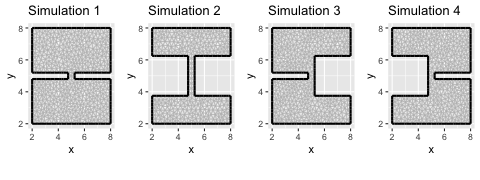
\includegraphics[width=1\linewidth]{bookdown-demo_files/figure-latex/squares-1} \caption{Delaunay triangulation for the different geometries used in simulations}\label{fig:squares}
\end{figure}

Simulations are done over a square shaped area, and two rectangular areas as barriers. The geometries of the barrier areas were changed in each simulation. Figure \ref{fig:squares} shows four different geometrical configurations for barrier areas. As mentioned before for each of these geometrical configurations different \(r_{b_2}\)´s were considered.

The range parameter on the left polygon was \(r_{b_1}\), and \(r_{b_2}\) on the right polygon in every scenario. The barrier polygons will be referred as \emph{left barrier} and \emph{right barrier} respectively. Moreover, priors are chosen arbitrarily, and INLA is run using a Gaussian likelihood. The model only takes an intercept and spatial effect \(f\) (this was referred to as model component in the previous section).

\begin{figure}
\centering
\includegraphics{bookdown-demo_files/figure-latex/gifs4-1.gif}
\caption{\label{fig:gifs4}Simulation scenario 1: row one shows the true simulated spatial field; row two and three the posterior mean for the transparent barrier model and the stationary model; and row four and five, the standard deviation for the transparent barrier model and the stationary model}
\end{figure}

\begin{table}

\caption{\label{tab:t1}summary of posterior range in the Transparent Barrier model for simulation geometry 1}
\centering
\begin{tabular}[t]{l|r|r|r}
\hline
r & mean & 0.025quant & 0.975quant\\
\hline
0.01 & 2.974864 & 1.852353 & 4.886259\\
\hline
\textasciitilde{}0.75 & 2.797209 & 1.821862 & 4.462563\\
\hline
\textasciitilde{}1.5 & 3.010664 & 1.729689 & 5.284214\\
\hline
\textasciitilde{}2.25 & 3.126231 & 1.729975 & 5.553413\\
\hline
3 & 3.541654 & 2.104981 & 6.257196\\
\hline
\end{tabular}
\end{table}

\begin{table}

\caption{\label{tab:t2}summary of posterior range in the stationary model for simulation geometry 1}
\centering
\begin{tabular}[t]{l|r|r|r}
\hline
r & mean & 0.025quant & 0.975quant\\
\hline
0.01 & 2.788175 & 1.652295 & 4.521668\\
\hline
\textasciitilde{}0.75 & 2.719023 & 1.682043 & 4.345092\\
\hline
\textasciitilde{}1.5 & 2.488462 & 1.450965 & 4.067897\\
\hline
\textasciitilde{}2.25 & 2.501149 & 1.312662 & 4.210762\\
\hline
3 & 3.137698 & 1.769617 & 5.287945\\
\hline
\end{tabular}
\end{table}

The simulated spatial field is compared with the results from the Transparent Barrier model and stationary model through the posterior mean and standard deviation as Figure \ref{fig:gifs4} shows. The simulated spatial field is shown in the first row of Figure \ref{fig:gifs4}, the posterior mean computed with the transparent barrier model and stationary model on row two and three, and the posterior standard deviation on row four and five (for the transparent barrier model and stationary model, respectively). The range parameters \(r_{b_2}\) used in the simulations are \(0.01\), \(\sim0.75\), \(\sim1.5\), \(\sim2.25\), \(3\) from left to right. Tables \ref{tab:t1} \ref{tab:t2} show the retrieved summary statistics for the posterior range parameter \(r_{b_2}\).Results for the other geometries are shown at the end of this section.

\begin{figure}
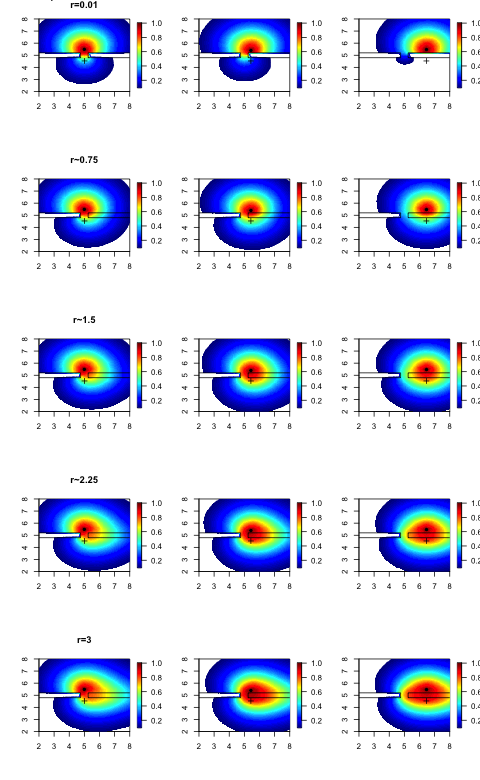
\includegraphics[width=0.5\linewidth]{bookdown-demo_files/figure-latex/circles4-1} \caption{Correlation structure of the trannsparent Barrier model with respect to specific points for simulation scenario 1.}\label{fig:circles4}
\end{figure}

\begin{figure}
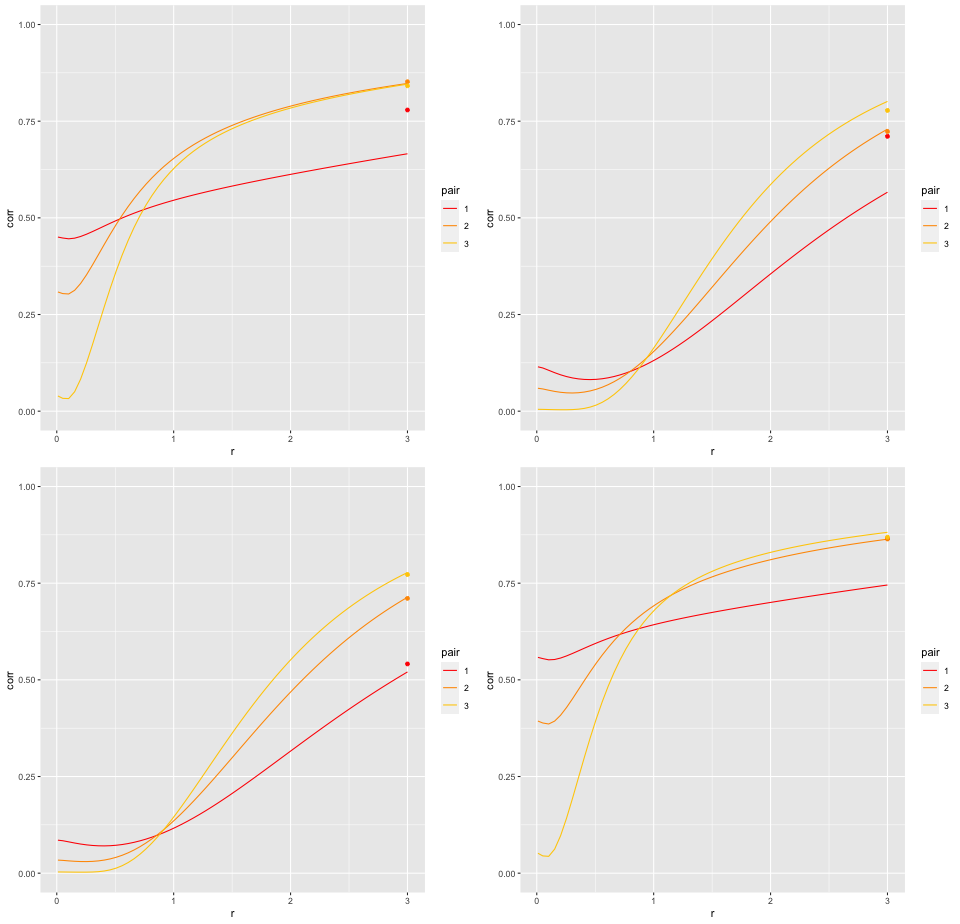
\includegraphics[width=13.33in]{bookdown-demo_files/figure-latex/pairs-1} \caption{Correlation curves between two points. The top left plot corresponds to simulation scenario 1; the top right to simulation scenario 2; the bottom left to the simulation scenario 3; and the bottom right to the simulation scenario 4. Pair 1, 2 and 3 correspond to locations taken in between barriers, on the edge of the right barrier or the middle of the right barrier, respectively. The dots in the plots correspond to the calculated correlation for a field with no barriers, i.e. where the range parameter is three everywhere.}\label{fig:pairs}
\end{figure}

To understand the effect of the range parameter on the correlation, points along side the right barrier are taken to compute the spatial correlation surface with respect to that point (Figure \ref{fig:circles4}, and the other scenarios at the end of this section). After doing so, locations on the other side of the barrier are taken (cross mark on Figure \ref{fig:circles4}) and correlation between these \emph{pair} of points is computed. Figure \ref{fig:pairs} shows the correlation curves for a pair of points taken from the the space in between barriers (\emph{pair 1}), on the edge of the right barrier (\emph{pair 2}), and at the middle of the right barrier (\emph{pair 3}). To get smoother curves \(60\) different \(r_{b_2}\) are used. Unlike the previous shown results all of the scenarios are plotted in Figure \ref{fig:pairs} (simulation scenarios 1 and 2 in the top left and right, respectively; and simulation scenarios 3 and 4 in the bottom left and right, respectively). Also shown here (as colored dots in each plot) is the correlation between the same pairs of points when there are no barriers, i.e.~\(r_n=r_{b_1}=r_{b_2}=3\) for each simulation scenario.

Pair 1, 2 and 3 correspond to locations taken in between barriers, on the edge of the right barrier or the middle of the right barrier, respectively. The dots in the plots correspond to the calculated correlation for a field with no barriers, i.e.~where the range parameter is three everywhere

\begin{figure}
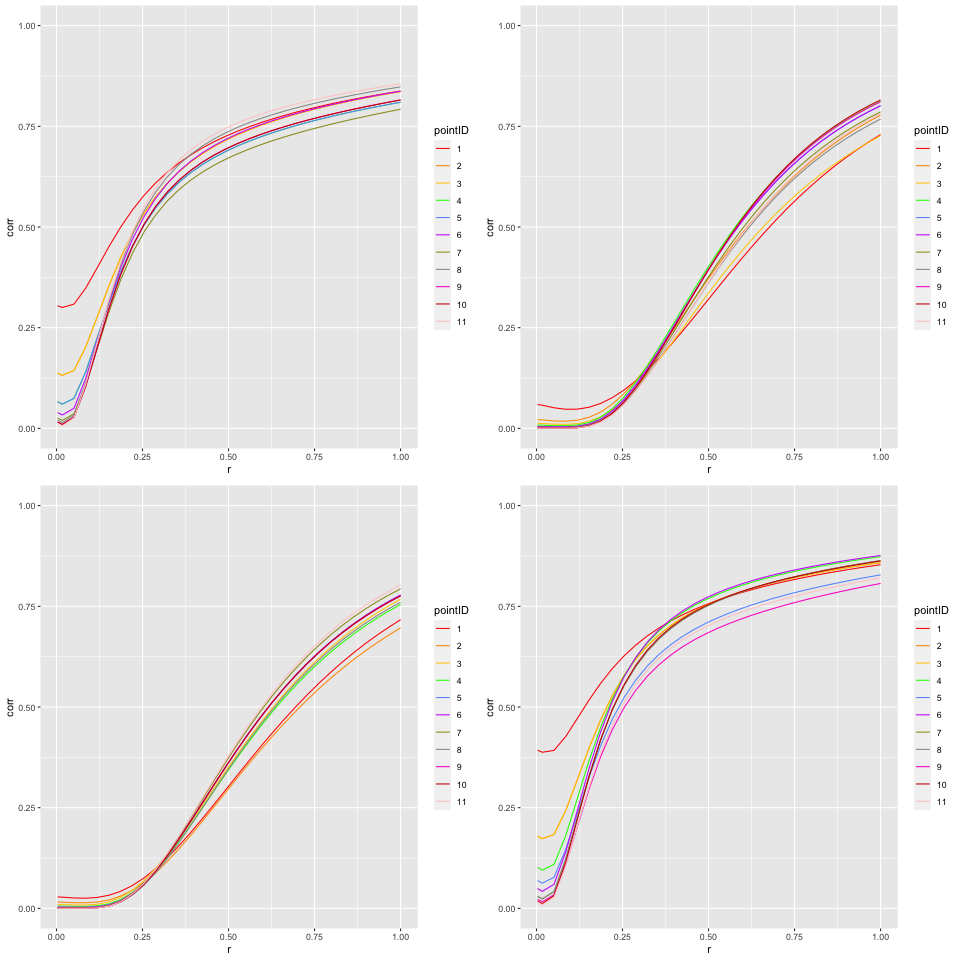
\includegraphics[width=13.33in]{bookdown-demo_files/figure-latex/corr11-1} \caption{Correlation curves between two points. The top left plot corresponds to simulation scenario 1; the top right to simulation scenario 2; the bottom left to the simulation scenario 3; and the bottom right to the simulation scenario 4. PointID 1 to 11 correspond to locations starting at 5.5 (pointID = 1) on the x-axis of the area of simulation, until 7.5 (pointID = 11) on the x-axis of the area of simulation. The range parameter is re-scaled so that the values are between 0 and 1.}\label{fig:corr11}
\end{figure}

\begin{figure}
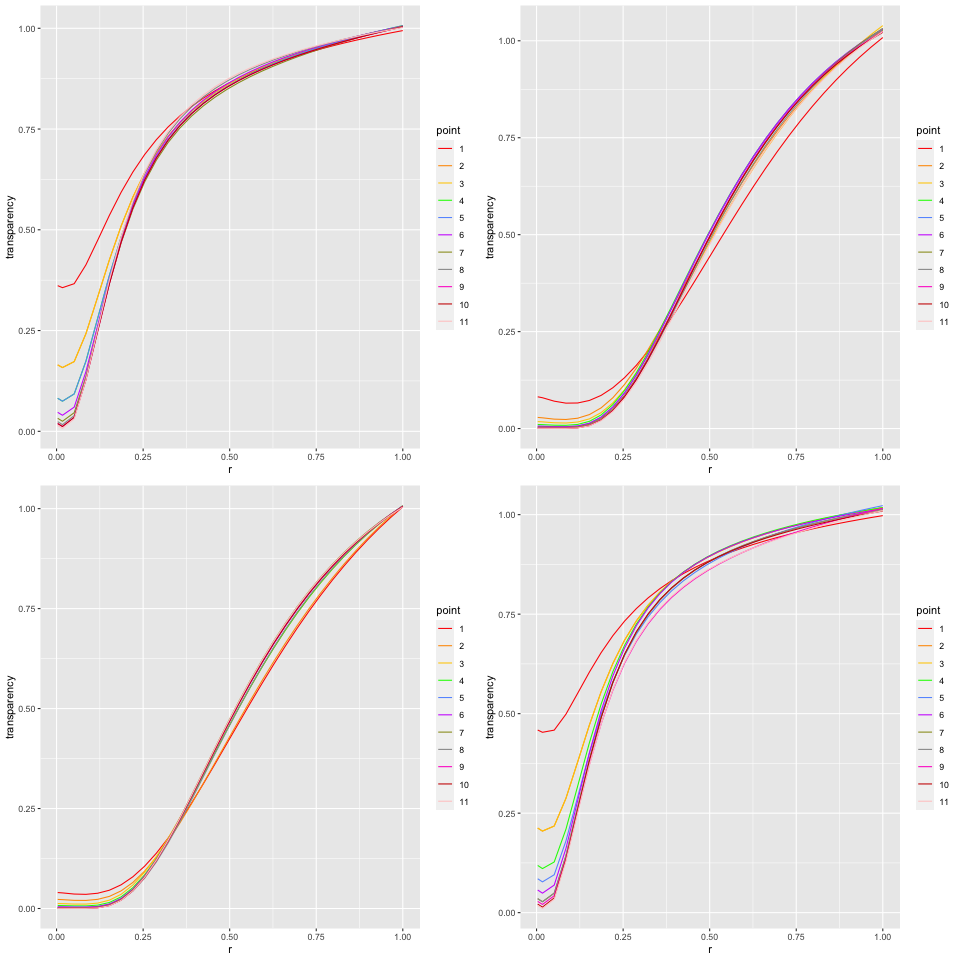
\includegraphics[width=13.33in]{bookdown-demo_files/figure-latex/trans11-1} \caption{Transparency curves. The top left plot corresponds to simulation scenario 1; the top right to simulation scenario 2; the bottom left to the simulation scenario 3; and the bottom right to the simulation scenario 4. PointID 1 to 11 correspond to locations starting at 5.5 (pointID = 1) on the x-axis of the area of simulation, until 7.5 (pointID = 11) on the x-axis of the area of simulation. The range parameter is re-scaled so that the values are between 0 and 1.}\label{fig:trans11}
\end{figure}

The same pairwise correlation is computed but considering eleven pairs from \(5.5\) to \(7.5\) along the \(x-axis\) of the big square area (Figure \ref{fig:corr11}). In other words these eleven pairs of points are centered in the right barrier area. The plot is done re-scaling the range parameter \(r_{b_2}\) to have it in a scale from \(0\) to \(1\), instead of \(0\) to \(3\).

Finally, for the same eleven pairs, \emph{transparency} values are computed dividing the correlation calculated between the two points by the correlation between those same two points as if no barriers existed. The results for all of the simulated scenarios are shown in Figure \ref{fig:trans11}.

\begin{figure}
\centering
\includegraphics{bookdown-demo_files/figure-latex/gifs25-1.gif}
\caption{\label{fig:gifs25}Simulation scenario 2: row one shows the true simulated spatial field; row two and three the posterior mean for the transparent barrier model and the stationary model; and row four and five, the standard deviation for the transparent barrier model and the stationary model}
\end{figure}

\begin{table}

\caption{\label{tab:unnamed-chunk-2}summary of posterior range in the Transparent Barrier model for simulation geometry 2}
\centering
\begin{tabular}[t]{l|r|r|r}
\hline
r & mean & 0.025quant & 0.975quant\\
\hline
0.01 & 3.203846 & 1.944570 & 5.390149\\
\hline
\textasciitilde{}0.75 & 3.563742 & 2.155955 & 6.021626\\
\hline
\textasciitilde{}1.5 & 2.876746 & 1.720469 & 4.876359\\
\hline
\textasciitilde{}2.25 & 3.648583 & 2.126992 & 6.761547\\
\hline
3 & 3.596270 & 2.118037 & 6.615297\\
\hline
\end{tabular}
\end{table}

\begin{table}

\caption{\label{tab:unnamed-chunk-3}summary of posterior range in the stationary model for simulation geometry 2}
\centering
\begin{tabular}[t]{l|r|r|r}
\hline
r & mean & 0.025quant & 0.975quant\\
\hline
0.01 & 3.439293 & 1.950754 & 5.802090\\
\hline
\textasciitilde{}0.75 & 4.282018 & 2.368254 & 7.470850\\
\hline
\textasciitilde{}1.5 & 3.431230 & 1.787240 & 5.962598\\
\hline
\textasciitilde{}2.25 & 5.050341 & 2.539630 & 9.804993\\
\hline
3 & 4.331167 & 2.287289 & 8.116793\\
\hline
\end{tabular}
\end{table}

\begin{figure}
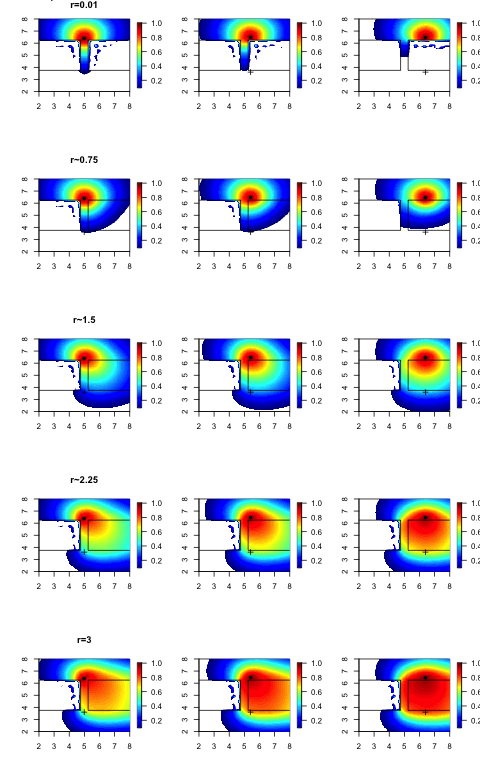
\includegraphics[width=0.5\linewidth]{bookdown-demo_files/figure-latex/unnamed-chunk-4-1} \caption{Correlation structure of the trannsparent Barrier model with respect to specific points for simulation scenario 2.}\label{fig:unnamed-chunk-4}
\end{figure}

\begin{figure}
\centering
\includegraphics{bookdown-demo_files/figure-latex/gifs425-1.gif}
\caption{\label{fig:gifs425}Simulation scenario 3: row one shows the true simulated spatial field; row two and three the posterior mean for the transparent barrier model and the stationary model; and row four and five, the standard deviation for the transparent barrier model and the stationary model}
\end{figure}

\begin{table}

\caption{\label{tab:unnamed-chunk-5}summary of posterior range in the Transparent Barrier model for simulation geometry 3}
\centering
\begin{tabular}[t]{l|r|r|r}
\hline
r & mean & 0.025quant & 0.975quant\\
\hline
0.01 & 3.603066 & 2.056069 & 6.364384\\
\hline
\textasciitilde{}0.75 & 4.345566 & 2.485301 & 8.187988\\
\hline
\textasciitilde{}1.5 & 4.142894 & 2.386104 & 7.826940\\
\hline
\textasciitilde{}2.25 & 3.058818 & 1.737644 & 5.475094\\
\hline
3 & 3.014614 & 1.739573 & 5.347236\\
\hline
\end{tabular}
\end{table}

\begin{table}

\caption{\label{tab:unnamed-chunk-6}summary of posterior range in the stationary model for simulation geometry 3}
\centering
\begin{tabular}[t]{l|r|r|r}
\hline
r & mean & 0.025quant & 0.975quant\\
\hline
0.01 & 3.597630 & 1.960700 & 6.193697\\
\hline
\textasciitilde{}0.75 & 3.863894 & 2.052807 & 6.951083\\
\hline
\textasciitilde{}1.5 & 3.799852 & 2.085991 & 6.853559\\
\hline
\textasciitilde{}2.25 & 2.773834 & 1.602145 & 4.635400\\
\hline
3 & 2.876769 & 1.548512 & 4.991123\\
\hline
\end{tabular}
\end{table}

\begin{figure}
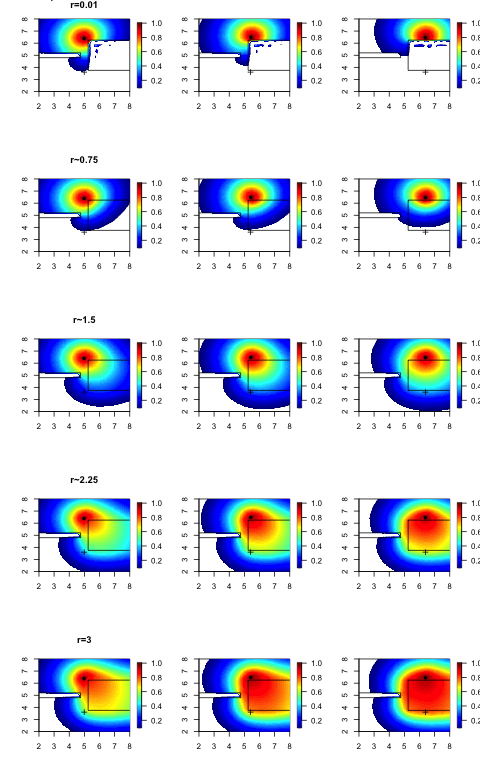
\includegraphics[width=0.5\linewidth]{bookdown-demo_files/figure-latex/unnamed-chunk-7-1} \caption{Correlation structure of the Transparent Barrier model with respect to specific points for simulation scenario 3.}\label{fig:unnamed-chunk-7}
\end{figure}

\begin{figure}
\centering
\includegraphics{bookdown-demo_files/figure-latex/gifs254-1.gif}
\caption{\label{fig:gifs254}Simulation scenario 4: row one shows the true simulated spatial field; row two and three the posterior mean for the transparent barrier model and the stationary model; and row four and five, the standard deviation for the transparent barrier model and the stationary model}
\end{figure}

\begin{table}

\caption{\label{tab:unnamed-chunk-8}summary of posterior range in the Transparent Barrier model for simulation geometry 4}
\centering
\begin{tabular}[t]{l|r|r|r}
\hline
r & mean & 0.025quant & 0.975quant\\
\hline
0.01 & 1.859714 & 1.144234 & 3.129831\\
\hline
\textasciitilde{}0.75 & 2.040998 & 1.266619 & 3.362025\\
\hline
\textasciitilde{}1.5 & 2.317718 & 1.333195 & 4.165207\\
\hline
\textasciitilde{}2.25 & 2.251755 & 1.328694 & 3.941123\\
\hline
3 & 2.328620 & 1.406326 & 3.946882\\
\hline
\end{tabular}
\end{table}

\begin{table}

\caption{\label{tab:unnamed-chunk-9}summary of posterior range in the stationary model for simulation geometry 4}
\centering
\begin{tabular}[t]{l|r|r|r}
\hline
r & mean & 0.025quant & 0.975quant\\
\hline
0.01 & 1.766470 & 1.043857 & 2.898305\\
\hline
\textasciitilde{}0.75 & 1.903328 & 1.175397 & 2.994670\\
\hline
\textasciitilde{}1.5 & 2.329499 & 1.251579 & 4.072913\\
\hline
\textasciitilde{}2.25 & 2.183446 & 1.249432 & 3.642843\\
\hline
3 & 2.311270 & 1.356024 & 3.784855\\
\hline
\end{tabular}
\end{table}

\begin{figure}
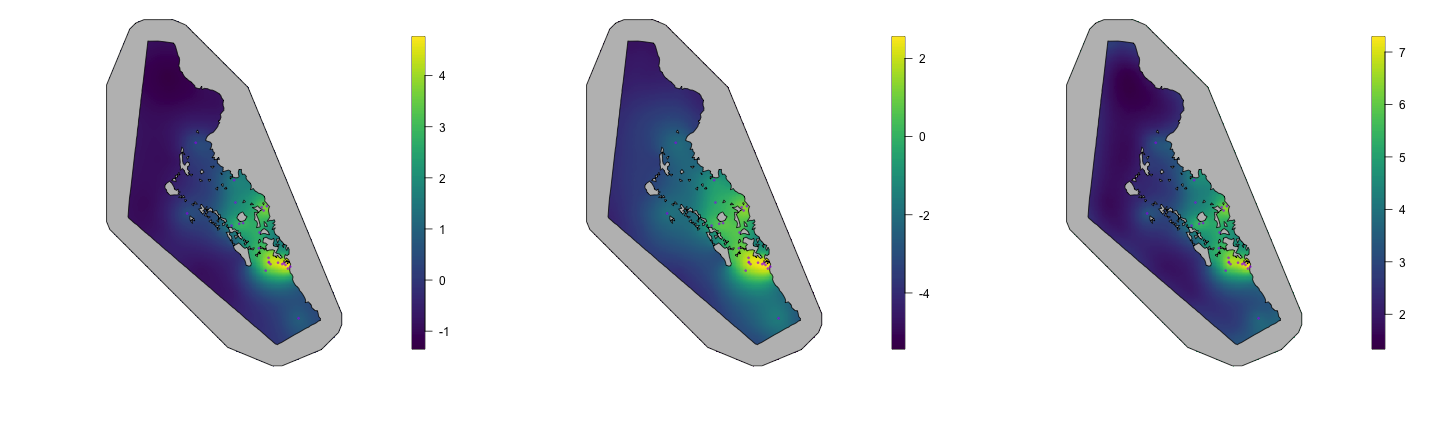
\includegraphics[width=0.5\linewidth]{bookdown-demo_files/figure-latex/unnamed-chunk-10-1} \caption{Correlation structure of the Transparent Barrier model with respect to specific points for simulation scenario 4.}\label{fig:unnamed-chunk-10}
\end{figure}

\hypertarget{discussion-and-future-work}{%
\section{Discussion and future work}\label{discussion-and-future-work}}

The study presents a significant outcome by successfully implementing the model within the Integrated Nested Laplace Approximation (INLA) framework. The results show the proposed Transparent Barrier model can handle complex spatial structures with diverse barriers, retaining computational efficiency inherent in stationary models. Comparative analysis with results from the stationary model reveals disparities, underscoring the importance of considering real-world scenarios with holes, barriers, or boundaries of varied nature.

While the current interpretation of parameters relies on intuition, forthcoming research will focus on mapping the range parameter \(r\) and developing a mathematical expression for \emph{transparency} with broader interpretability, reducing its dependence on specific cases, be they simulated or from real-life applications.

The ultimate phase of this project will involve an application of INLA to facilitate accessibility and practical implementation of the Transparent Barrier model.

\hypertarget{megafauna-application}{%
\chapter{Megafauna application}\label{megafauna-application}}

\hypertarget{motivation-1}{%
\section{Motivation}\label{motivation-1}}

Certainly marine megafauna play crucial roles in marine ecosystems, contributing to their health and functioning.
Marine megafauna, such as whales, sharks, and large rays, are often considered keystone species \citep{hooper_effects_2005}. They have a disproportionate impact on their ecosystems, influencing the abundance and distribution of other species. For example, whales contribute to nutrient cycling through their fecal plumes, enhancing primary productivity \citep{estes_trophic_2011}. Their presence is also associated with higher biodiversity levels because interactions with other species, such as fish and invertebrates, create complex ecological relationships \citep{beger_conservation_2010, block_tracking_2011, heithaus_predicting_2008, orams_marine_2002}.

Conservation efforts focused on these species are crucial not only for their survival but also for the overall health and resilience of marine ecosystems. Appropriate management plans can vary drastically depending on specific contributions of marine megafauna based on the species and the characteristics of the ecosystems they inhabit. Equally relevant is the variability of potential management plans that can be considered due to socioeconomic characteristics of potential conservation areas, e.g.~coastal areas dedicated for tourism, fishery or channel from oil plants to oil refinement facilities will require different management plans since most of the times human activity cannot be reduced drastically. Therefore, it is key to count with Spatial Distribution Models (SDMs) that can be used at local scale to properly manage areas of interest.

Spatial distribution models play a pivotal role in scientific research focused on marine megafauna, aiding in the understanding of species distribution, interactions, and the ecological significance of specific areas. One prominent approach is the use of Species Distribution Models (SDMs), which aim to predict the spatial distribution of marine megafauna based on environmental variables. These models establish statistical relationships between species occurrence data and predictors like temperature and ocean currents, employing algorithms such as MaxEnt, Random Forest, and Generalized Additive Models (GAMs). SDMs help assess potential distribution, identify critical habitats, and project responses to environmental changes. However, these models heavily rely on the quality and representativeness of input data for the explanatory environmental variables, and the sample size. Some, like MaxEnt, also present the challenge of not modeling count data explicitly and only do so through pseudo-absence techniques.

Consequentely, when environmental data is not complete or its not sufficient to explain the variation, SDMs that can incorporate spatial random effects for unexplained spatial dependence need to be considered. Notice that even if there is enough data on environmental explanatory variables some other underlying processes may affect species distributions. For example some intrinsic inter-specific process.

Even in an SDM framework that explicitly incorporates spatial random effects another problem is encountered. SDMs (usually) assume that the spatial random effect is stationary and isotropic (both together usually referred as stationarity). Implying the random effect remains unchanged when the underlying map is rotated, i.e.~correlation only depends on the distance and not on the spatial coordinates. In study areas where there are physical barriers the latter is not the case.

Stationarity assumptions are more often than not, unrealistic in coastal areas where, by definition, the coast represents a physical barrier for marine species. Moreover, considering that there is more than one \emph{type} of barrier is reasonable. In the same coastal area for example, there might be sand or rocky patches that present barriers that, unlike the coast, might be crossed from time to time. Then there is an \emph{impermeable} barrier, the coast, and some other barriers with varying permeability.

The intention in this chapter is to model the distribution of Dugongs (\emph{Dugong dugon}) in the northern coast of the Saudi Arabian Red Sea considering this is an area with islands and sand patches. The ultimate goal is to provide Red Sea Global (RSC) and Amaala projects with marine megafauna species distribution models for their protection in the area where these two projects are located \citep{public_investment_fund_red_2018, public_investment_fund_amaala_2018}.

\hypertarget{saudi-arabian-red-sea-coast}{%
\section{Saudi Arabian Red Sea coast}\label{saudi-arabian-red-sea-coast}}

As mentioned, the Red Sea has a complex spatial structure with lots of islands along the coast. Moreover, the information available is not precise when it comes to showing these islands on the map so when the Dugong data was first analyzed lots of questions arise. This is what ultimately led to the entirety of this research project.

The data comes from incidental Dugong sightings. Incidental sighting refers to observations that are recorded opportunistically or incidentally, often without a pre-planned sampling design. Unlike systematic surveys or dedicated monitoring efforts, incidental sighting data are collected as a byproduct of other activities, such as tourism, research cruises, or citizen science initiatives. Incidental sighting data, being count data, can be conceptualized within the framework of a Poisson point process when modeling the spatial distribution of Dugong (or any other species) occurrences. The Poisson process provides a mathematical foundation to describe the occurrence of random events in continuous time or space (\emph{Introduction} section has a more detailed definition). Additional to the Dugong data, bathymetry data for the study area was given by the RSC project.

\begin{figure}
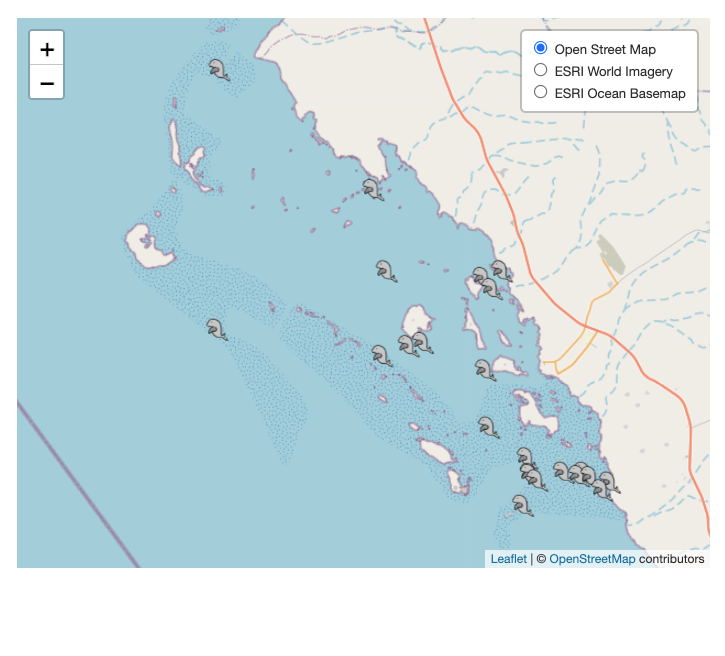
\includegraphics[width=0.7\linewidth]{bookdown-demo_files/figure-latex/plot1-1} \caption{Study area. On the right plot the blue polygon on top of the study area shows sea area according to the only available map considering islands.}\label{fig:plot1}
\end{figure}

\begin{figure}
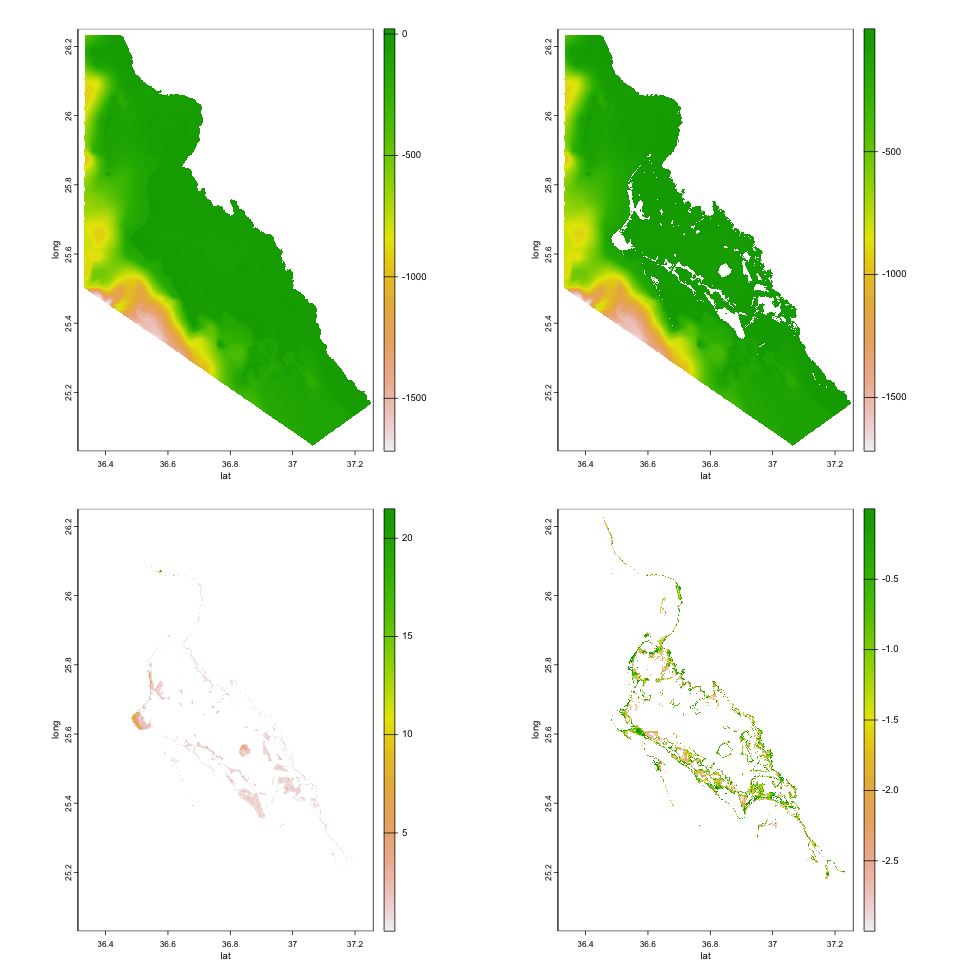
\includegraphics[width=0.7\linewidth]{bookdown-demo_files/figure-latex/bathym0-1} \caption{Bathymetry map for the the entire study area on the left, and the area excluding islands on the right.}\label{fig:bathym0}
\end{figure}

Figure \ref{fig:plot1} shows the study area and locations of the Dugong sightings. Adding to the difficulty of the area given by the islands, there are no precise maps that display them. Quite the opposite, the available map considering islands grouped them together so that combining the map with the Dugong locations one observation is on land (Figure \ref{fig:plot1} right plot). Because of it bathymetry data was used to construct a map instead of incorporating it as a fixed effect in the model. Islands were taken to be bathymetry values greater or equal to \(0\) (Figure \ref{fig:plot1}).

\hypertarget{barrier-model}{%
\section{Barrier model}\label{barrier-model}}

All models are fitted in INLA considering a Bayesian spatial model under the Barrier model and LGCP framework \citep{bakka_non-stationary_2019, krainski_advanced_2018, simpson_going_2016} is used to fit the data. Accordingly, the response variable is assumed to have a Poisson distribution with intensity \(\lambda_A=\int_A \lambda(\mathbf{s}) d \mathbf{s}\), and \[\log (\lambda(\mathbf{s}))=\beta_0+u(\mathbf{s})\], with \(\beta_0\) the intercept and \(u(\mathbf{s})\) the random effect.

\[\begin{aligned}
& x(s)-\nabla \cdot \frac{r_n^2}{8} \nabla x(s)=r_n \sqrt{\frac{\pi}{2}} \sigma_x \mathcal{W}(s), \text { for } s \in \Omega_n \\
& x(s)-\nabla \cdot \frac{r_b^2}{8} \nabla x(s)=r_b \sqrt{\frac{\pi}{2}} \sigma_x \mathcal{W}(s), \text { for } s \in \Omega_b,
\end{aligned}\]

where \(r_n\) is the range parameter for the sea area, \(r_b\) is the range parameter for the island barrier area, \(\Omega_n\) is the sea area, and \(\Omega_b\) the island area. The disjoint union of both \(\Omega_n\) and \(\Omega_b\) gives the whole study area \(\Omega\). More specifically, \(r_n=10\), and \(r_b=0.01\) are used.

A detailed explanation on the model construction is given in the previous section \emph{Transparent Barrier model} under \emph{Barrier model background}.

\begin{figure}
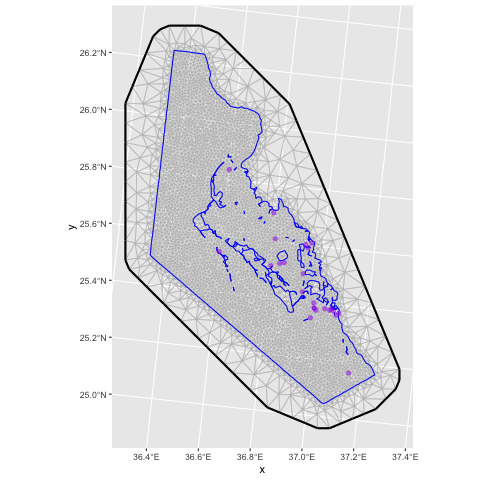
\includegraphics[width=0.4\linewidth]{bookdown-demo_files/figure-latex/mesh-1} \caption{Triangulation used to get the spatial field using the SPDE approach. The mesh built over the study area with purple dots representing the sightings.}\label{fig:mesh}
\end{figure}

Map of the study area with sightings locations (red dots). Triangulation used to calculate the GMRF for the SPDE approach. (For interpretation of the references to colour in this figure legend, the reader is referred to the web version of this article.)

Following the SPDE approach to fit an LGCP model the model is defined at mesh nodes (Figure \ref{fig:mesh}), and the expected number of events is to be proportional to the area around it, i.e.~nodes in larger triangles have greater expected values \citep{krainski_advanced_2018, simpson_going_2016}. PC-priors are defined on the hyper-parameters \(\sigma_u\) and \(r\) according to \citet{fuglstad_constructing_2019}, and the spatial effect depends only depends on these two unknown parameters. The fixed range close to \(0\) in the barrier results in local averaging in the sea so the dependency moves around the barrier.

The SPDE approach for point pattern analysis defines the model at the nodes of the mesh. To fit the log-Cox point process model, these points are considered as integration points. The method in \citet{simpson_going_2016} defines the expected number of events to be proportional to the area around the node (the areas of the polygons in the dual mesh). This means that at the nodes of the mesh with larger triangles, there are also larger expected values.

\hypertarget{results}{%
\section{Results}\label{results}}

\begin{figure}
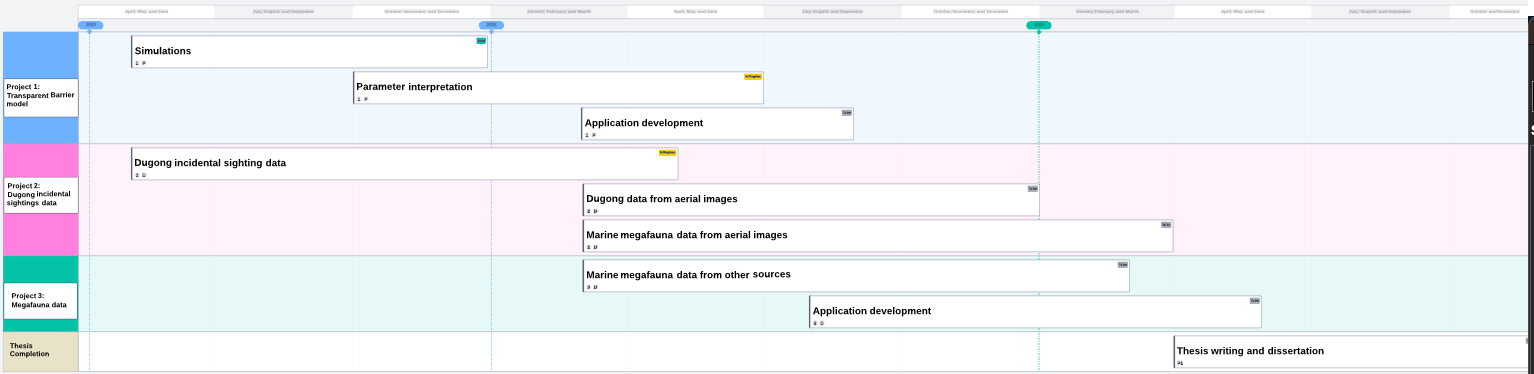
\includegraphics[width=1\linewidth]{bookdown-demo_files/figure-latex/unnamed-chunk-11-1} \caption{Posterior distribution for the mean on the left, 0.025 quantile on the middle, and 0.025 quantile on the right.}\label{fig:unnamed-chunk-11}
\end{figure}

Bayesian posterior distributions provide a straightforward way to make probability statements about unknown parameters so the region between 0.025 to 0.975 quantiles of the posterior distribution indicates a 95\% probability that the unknown parameter lies within this range of values.

\begin{figure}
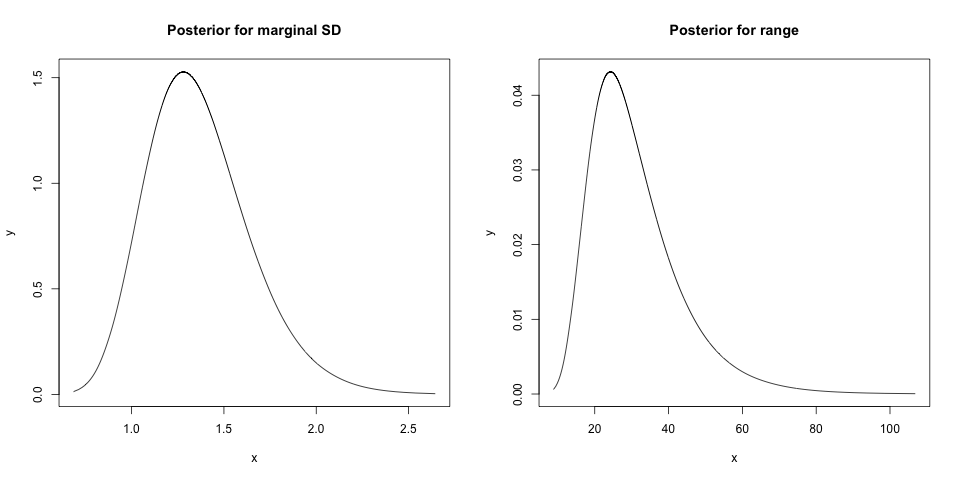
\includegraphics[width=0.5\linewidth]{bookdown-demo_files/figure-latex/hypermarginals-1} \caption{Posterior marginals for hyper-parameters of the model. On the left the standard deviation of the spatial effect, and on the right range of the sea (normal) area}\label{fig:hypermarginals}
\end{figure}

\begin{figure}
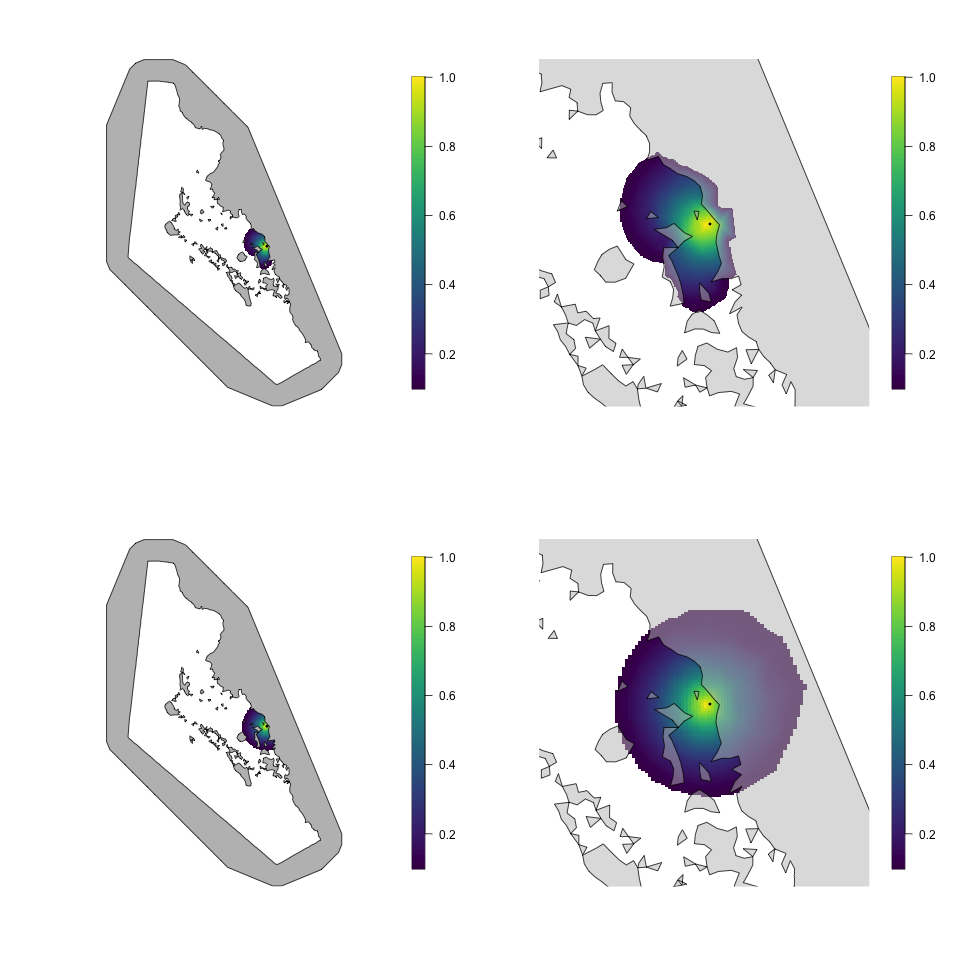
\includegraphics[width=0.7\linewidth]{bookdown-demo_files/figure-latex/fieldforpoint-1} \caption{Correlation structure with respect to one point obtained with the Barrier model (top row) and the stationary model (bottom row) to compare the work done here and the alternative assuming stationarity.}\label{fig:fieldforpoint}
\end{figure}

\hypertarget{discussion-an-future-work}{%
\section{Discussion an future work}\label{discussion-an-future-work}}

\begin{figure}
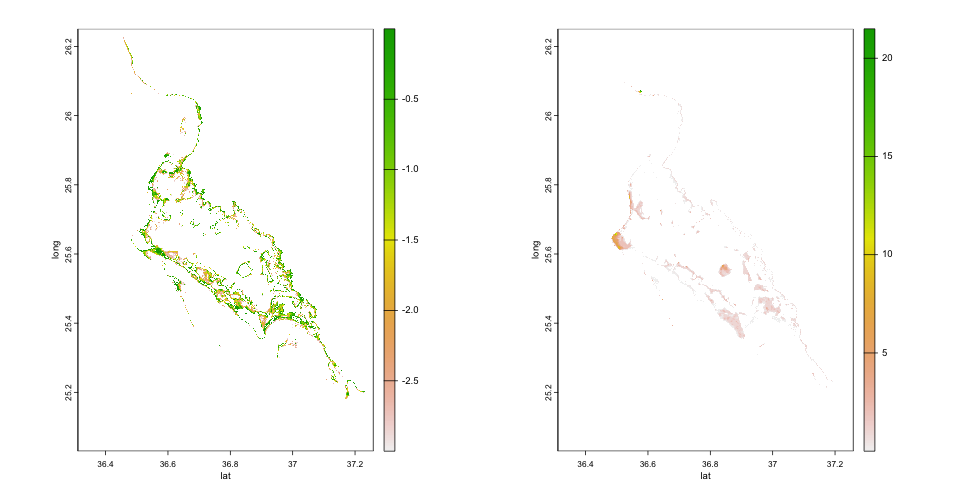
\includegraphics[width=1\linewidth]{bookdown-demo_files/figure-latex/bathy3-1} \caption{Bathymetry map for the entire area on the left, sand patches on the middle and islands on the right.}\label{fig:bathy3}
\end{figure}

As it can be seen the data has a few points so drawing conclusions doesn´t seem realistic. However, the complexity of the area makes trying different models interesting. Moreover, current focus is on taking not only islands as barriers, but islands and sand patches. Figure \ref{fig:bathy3} shows island regions (rightmost plot), and sand patches (middle plot) drawn from the bathymetry map. Sand patches were taken to be areas from \(0\) to \(3\) meters below sea level, the value \emph{3} is chosen arbitrarily, and it is only for illustration purposes. However, from this illustration it becomes apparent that the use of another barrier is needed since it can be seen that patches between \(0\) and \(1\) meter below the sea surround sea area leaving them potentially inaccessible for Dugongs.

The dataset utilized in this study was provided by the RSG project, serving as a preliminary exploration while they continue to gather more comprehensive data through drone and plane imaging. Subsequent efforts in this project will be directed towards the application of our model to newly acquired Dugong data and extending its applicability to videos capturing other species of interest.

A crucial aspect of our future work involves enhancing the interpretability of model parameters from both mathematical and applied perspectives. Continuous \emph{feedback} between this project and the previous one are integral, as it is necessary to make sense of the parameters from both the mathematical point of view and then applied point of view. We aim to provide guidance on selecting range parameters within barriers, making the model accessible for broader usage, and introducing the concept of transparency in real-life applications.

Conclusively, our project aims to establish a robust framework capable of handling multiple barrier types and varying levels of transparency, ensuring its versatility and effectiveness in diverse environmental applications.

\hypertarget{survey-data-application}{%
\chapter{Survey data application}\label{survey-data-application}}

\hypertarget{background-and-future-work}{%
\section{Background and future work}\label{background-and-future-work}}

\hypertarget{sampling-schemes.}{%
\subsection{Sampling schemes.}\label{sampling-schemes.}}

In marine megafauna scientific research, survey sampling methods from boats or planes are crucial for studying and monitoring large marine species. Common sampling schemes are summarized next.

\emph{Line Transect Surveys:} Line transect surveys involve navigating predetermined transect lines on a boat, with observers recording sightings of marine megafauna within a specified distance perpendicular to the transect line. In this methodology, researchers typically move along straight or zigzag transect lines, and observers note the distance and angle of each sighting from the transect line. The collected data includes species identification, group size, and perpendicular distance. Line transect surveys are commonly employed for estimating population density and abundance of species visible at the water's surface. They are also instrumental in calculating detection probabilities and adjusting for potential biases in estimates.

\emph{Point Transect Surveys:} Point transect surveys provide a more flexible approach compared to continuous line transects. In this method, sightings of marine megafauna are recorded at specific points along transect lines. Observers stationed at these points use equipment like rangefinders to measure distances to observed animals. The collected data include species identification, distance, and angle from each point. Point transect surveys are particularly useful for estimating detection functions and deriving abundance estimates. They offer enhanced precision in abundance estimates when accurate distance measurements are feasible, allowing for a more adaptable survey strategy.

\emph{Aerial Surveys:} Aerial surveys involve the use of aircraft to observe marine megafauna from an elevated perspective, covering large areas efficiently. Aircraft follow predetermined flight paths or grids, and observers aboard the aircraft record sightings of marine megafauna. Additionally, aerial photography or digital imaging may be employed for documentation purposes. Aerial surveys are known for efficiently surveying vast ocean areas, making them especially suitable for species like whales and dolphins. They provide valuable data on species distribution, abundance, and behavior, offering a unique and comprehensive perspective for research and conservation purposes.

\hypertarget{distance-sampling-frameworks}{%
\subsection{Distance sampling frameworks}\label{distance-sampling-frameworks}}

Understanding the spatial distribution and abundance of marine megafauna is essential for effective conservation and management strategies. Boat surveys utilizing line transects have become a widely employed method in ecological studies, providing valuable data for estimating population density.

Point processes are used to characterize the spatial distribution of marine megafauna individuals along transect . To do so detection functions are fundamental components within distance sampling models, capturing the probability of detecting an individual based on its distance from the observer or transect line. The choice of detection function, be it half-normal, hazard-rate, or negative exponential, significantly influences the accuracy of detection probability estimates. Moreover, recognizing the variability in detection probabilities with distance is crucial in distance sampling models. Statistical approaches explicitly account for the fact that not all individuals within the detection strip width are observed, and detection probability is often modeled as a function of distance \citep{ackerman_aerial_nodate, aguero-valverde_direct_2014, alves_aerial_2013, buckland_distance_2015}.

\hypertarget{future-work}{%
\subsection{Future work}\label{future-work}}

The project aims to implement the Transparent Barrier model within the distance sampling framework.

  \bibliography{book.bib,packages.bib,Library.bib}

\end{document}
